
\section{Evaluation}

\subsection{Goodness of fit function}

It follows from the previous section that designing a filter entails a trade-off between the accuracy of the response of the passband, the transition zone, and the stopband. Different applications will therefore require different methods to assess the efficacy of a filter. The most common alternative for this is to compare the Fourier amplitude spectra. This  evaluation is typically done visually. We, however, seek to define standards that provide a solid reference framework for simulation validation. That is, we are interested in filters that are good for narrow bands at low frequencies and wider bands at higher frequencies, with sharp transition zones (sharp cut off frequency is better), minimum ripples in the passband amplitudes, and with sufficient attenuation in the stopbands (see Figure 4). In the context of the GOF analysis, \citet{Anderson_2004} defined the expression to evaluate the similarity between two Fourier amplitude spectra as:
% 
\begin{equation}
    \label{eq:s}
	S \left( p_1,p_2 \right) = 10 \exp \left\{ -\left[ \frac{p_1-p_2}{min \left(p_1,p_2\right)} \right]^2 \right\} 
    \hspace{0.25em},
\end{equation}
% 
Where $p_1$ and $p_2$ are the frequency amplitude of two waveforms evaluated at every frequency. Since the Fourier amplitude score in Anderson?s GOF method is the least sensitive parameter to filtering, we are interested in using a similar function to evaluate the filters? selection. Eq. (2) decreases monotonically as the difference between the parameters p1 and p2 increases. While this offers a good measure for almost all scales, it cannot characterize the differences when one of the parameters vanishes (becomes zero). This is important because in order to quantify the efficacy of the filtering process, we also need to consider the values in the stop band, which should be compared to zero. \citet{Khoshenvis_2015} defined complementary goodness of fit function for outside of the pass band where the ideal filter?s magnitude response is zero. 
% 
\begin{equation} 
    \label{eq:s-modified}
    S \left( p_1,p_2 \right) = 10 \exp \left\{ -\left[ \frac{p_1 - p_2}{F(a)} \right]^2 \right\} 
    \hspace{0.25em},
\end{equation}
% 
where $F(a)$ is a function of the amplitude inside the passband. The scoring scale defined by Eq. (3) avoids the division by zero and yet offers a signal specific measure of the accuracy of the filter with respect to an ideal filter with amplitude zero in the stopbands. We use Eq. (2) and Eq. (3) to evaluate the efficacy of filters by comparing the Fourier amplitudes of filtered signals with respect to the result that would be expected from an ideal filter, where the amplitude in the passband is the same amplitude of the original signal within the cutoff frequencies, and zero elsewhere. 

Figure 5 shows an example of this comparison and the resulting scores, using Eq. (2) for scoring the amplitude similarity in the passband and Eq. (3) for scoring the filtered signal remnant amplitude in the stopbands. The whole domain for comparing is max 1 Hz above and below the cutoff frequencies. In this study we assumed F(a) is a fraction of the average amplitude inside the band.
% 
\begin{equation}
    F(a) = C *  \mathrm{mean} \left( [f_1,f_2] \right)
    \hspace{0.25em}.
\end{equation}
% 
The values are computed for each discrete frequency and the final score is the mean of  the score at all frequencies within the comparison range.  

\begin{figure}
    \centering
    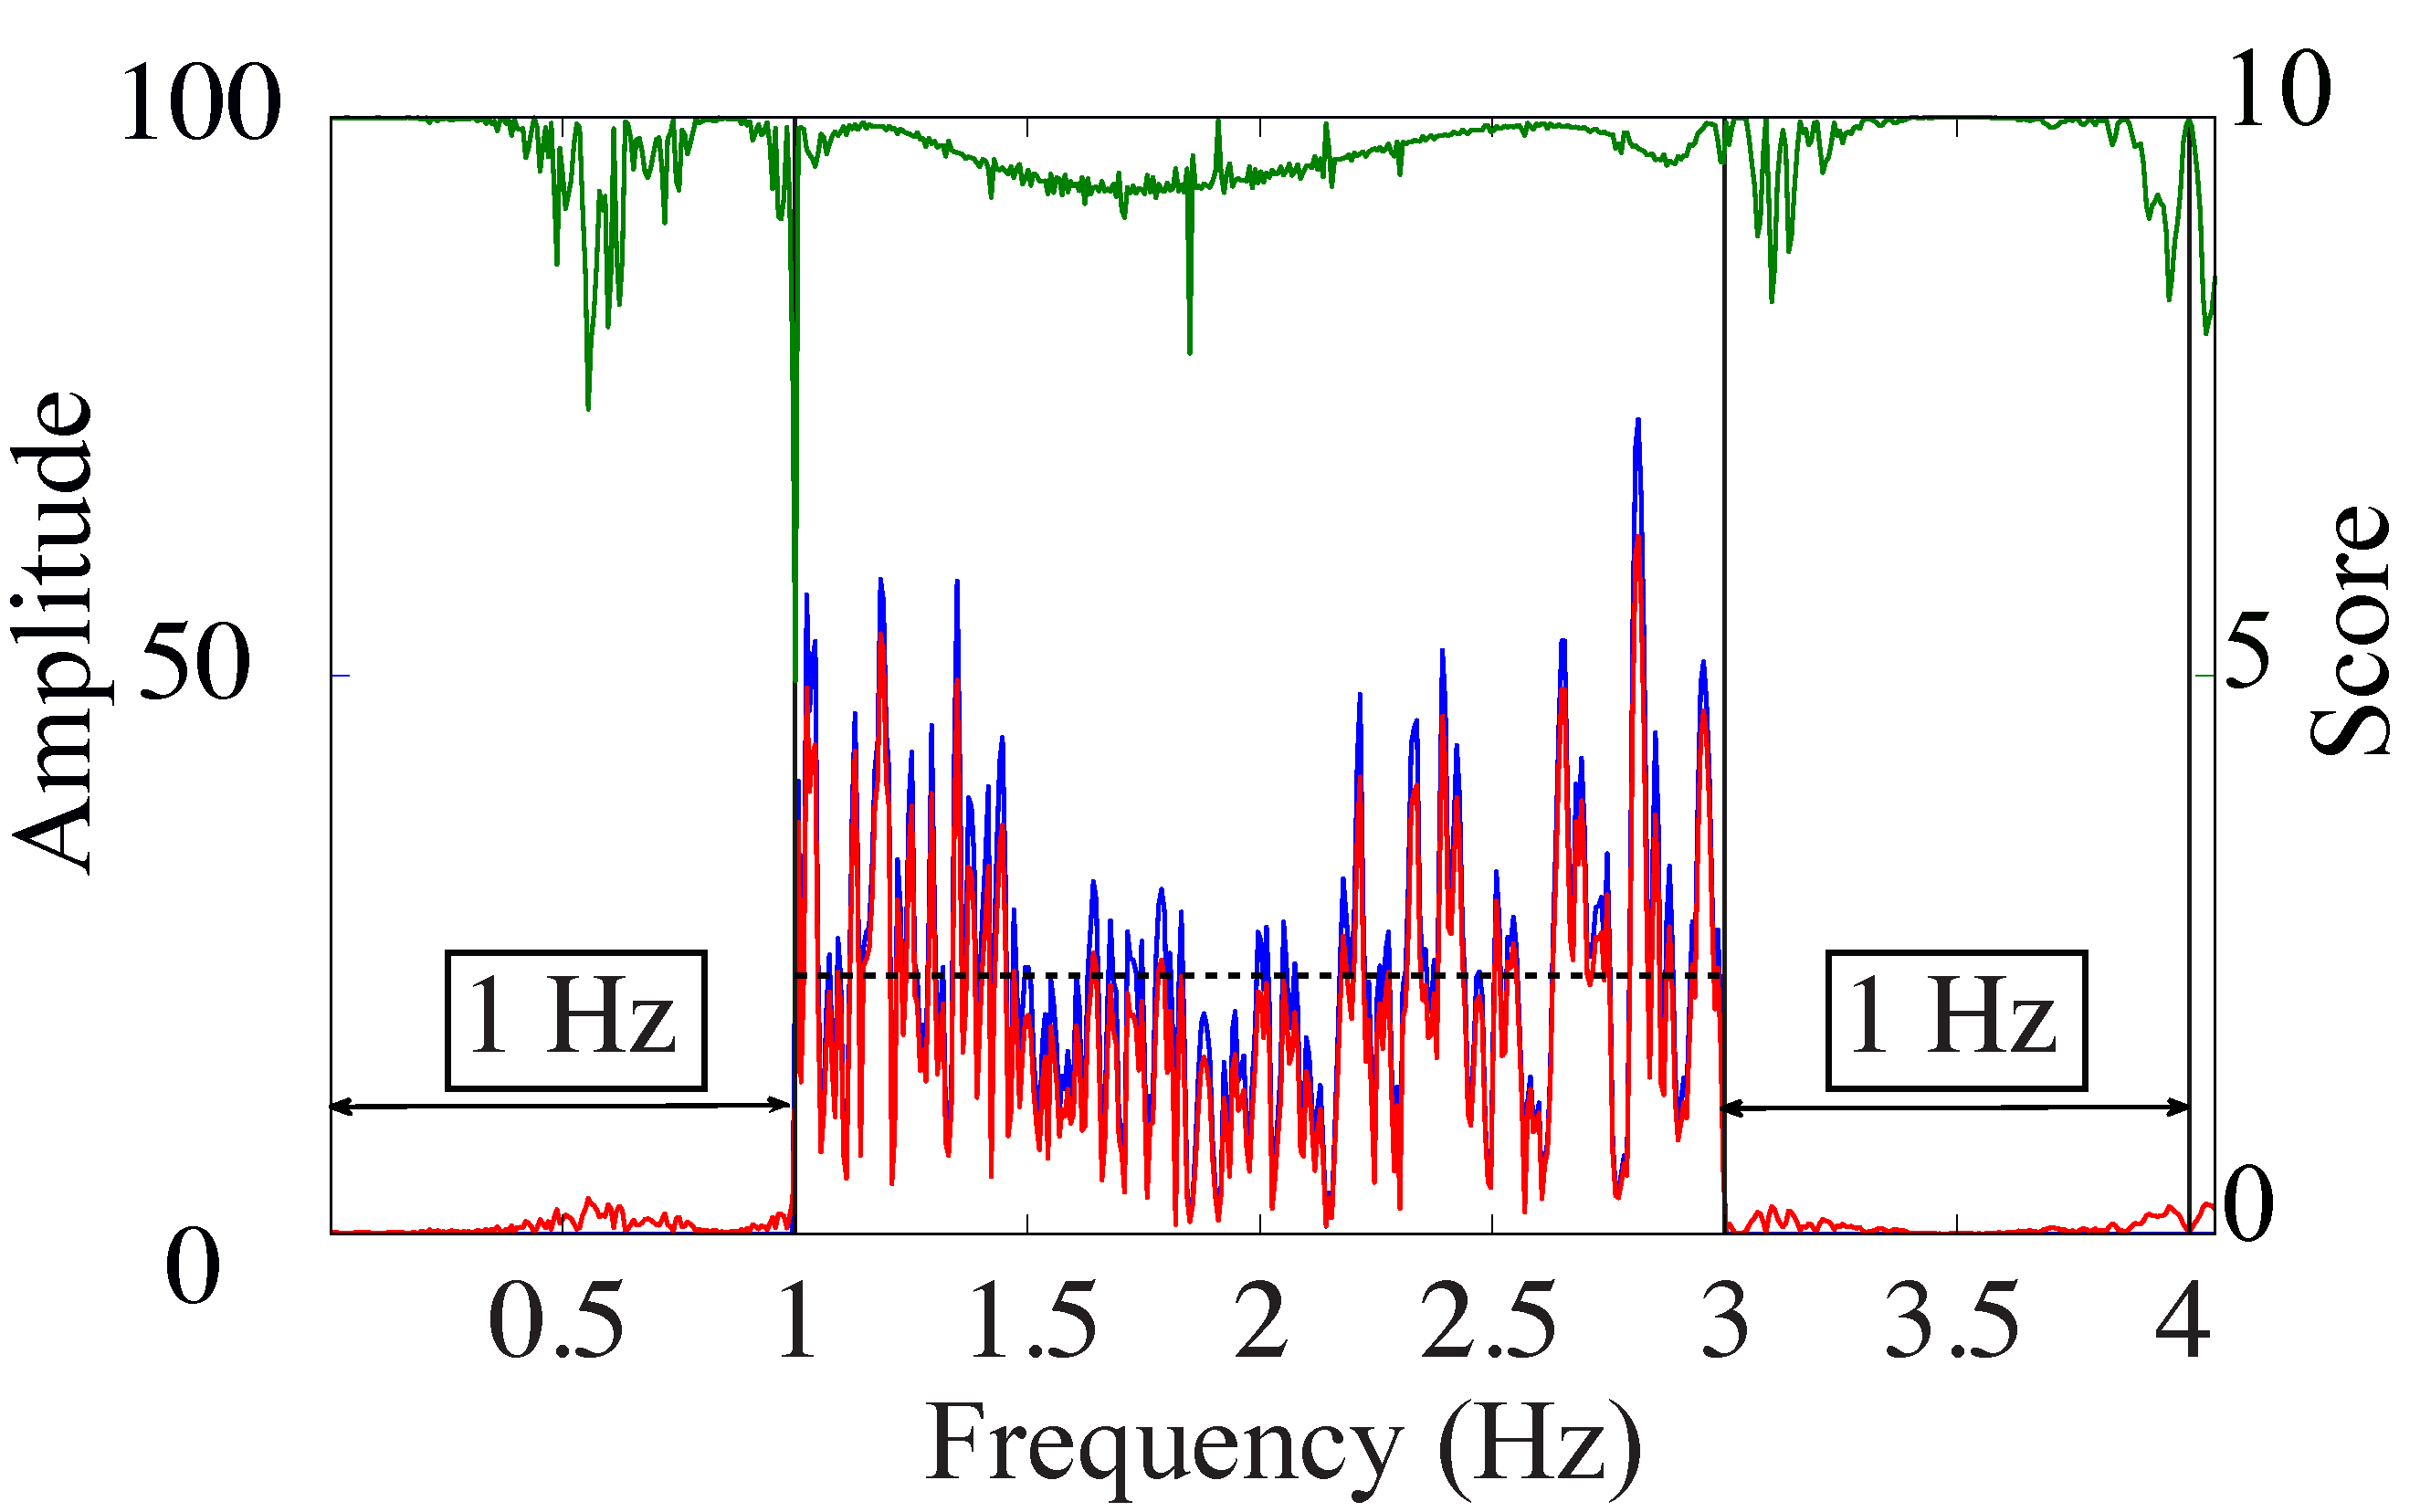
\includegraphics
    	[width=\mycolumnwidth]
    	{figures/pdf/figure5.pdf} 
    \caption{Evaluation of coherency between the ideal frequency response and filtered signal?s response. Left vertical axes is the amplitude and right vertical axes is the score. The mean of amplitude in the inside section is shown as dashed line.}
\end{figure}

Figure 6 illustrates the sensitivity of the score with changing $F(a)$. In this study we are looking for making a good balance between inside and outside of the band and non of them are dominant unless because of width. Decreasing the value to very low numbers less than (0.2) will make the score of some points very low, which cause unrealistic low score and will affect the broadband score, whereas  we may have good score inside the band. Very high values (higher than 0.4), will make the score very close to 10. This situation affects the functionality of  cost function of GA alghorithm, and make it less sensitive to the other parameters. Even though these numbers are different for different waveforms but the decreasing pattern is the same. We found that 0.25 * mean of inside the band gives good measure to handle the outside of the band according to the average amplitude of the passband.

\begin{figure}
    \centering
    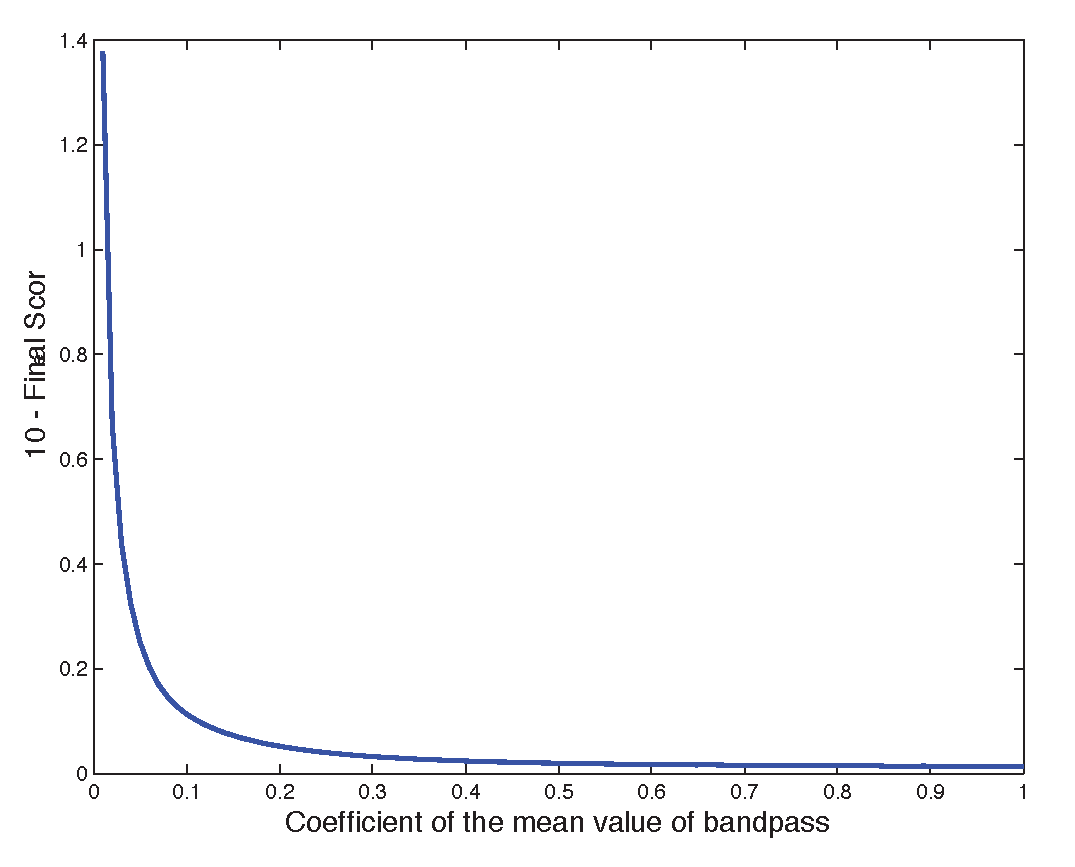
\includegraphics
    	[width=\mycolumnwidth]
    	{figures/pdf/figure6.pdf} 
    \caption{Sensitivity of final score to the coefficient of  goodness of fit criteria outside of the filtering band.}
\end{figure}

\subsection{Optimization alghorithm to find the best parameters}

In this paper we use  Genetic algorithms  (GA) to find the best parameters that results minimum residual than ideal filter. \citet{Holland_1973} introduced genetic algorithms; it is popular till, although it is slower than modified versions; designing efficient algorithm is not objective in this study. GA is not mathematically guided solution to the problem. It is merely a stochastic, discrete, nonlinear, and highly dimensional search algorithm.

Regarding the trade of entity of ideal filter between paramters, it is common to achevie good score based on different set of parameters,GA has the ability to solve multimodel problem with relative ease. We developed a simple GA  according \citet{Man_1996}. Each population has filters parameters. It is different for different filters. For elliptic filter it has 3 parameters ($LP_O$: order, $LP_RP$: peak to peak passband ripple, $LP_RS$: Stopband attenuation), $LP$ and $HP$ stands for lowpass stands for lowpass and highpass filter. butterworth filter has one parameter (order) and Chebyshev type 1 filter has 2 parameters (Order and peak to peak passband ripple).   The algorithm iteratively defines new populations whose filtered frequency components closely match the ideal frequency component. Every time that new population is generated it went through the evaluation process. In the evaluation process which we call it cost or objective function (according to GA nomencluter), it get the parameters as an input and design a filter based on that parameters. It filter the wave with the designed filter and take Fourier transform. It also take Fourier transform of original waveform and cut the stopnband part in amplitude (see figure 5). Then we evaluate two points at each frequency according to these conditions:
% 
\begin{equation}
	\left\{
		\begin{matrix}
			S \left( p_1,p_2 \right) = 
				10 \exp \left\{ -\left[ \frac{p_1-p_2}{min \left(p_1,p_2\right)} \right]^2 \right\} 
				& (p_1 > 0.0001) \& (p2 > 0.0001) \\   

			S \left( p_1,p_2 \right) = 
				10 \exp \left\{ -\left[ \frac{p_1 - p_2}{F(a)} \right]^2 \right\}
				& (p_1 > 0.0001) \& (p2 < 0.0001) || (p_1 < 0.0001) \& (p2 > 0.0001)\\

			S \left( p_1,p_2 \right) = 
				10  
				& (p_1 < 0.0001) \& (p2 < 0.0001) \\
		\end{matrix}
	\right.
\end{equation}

\begin{figure*}
    \centering
    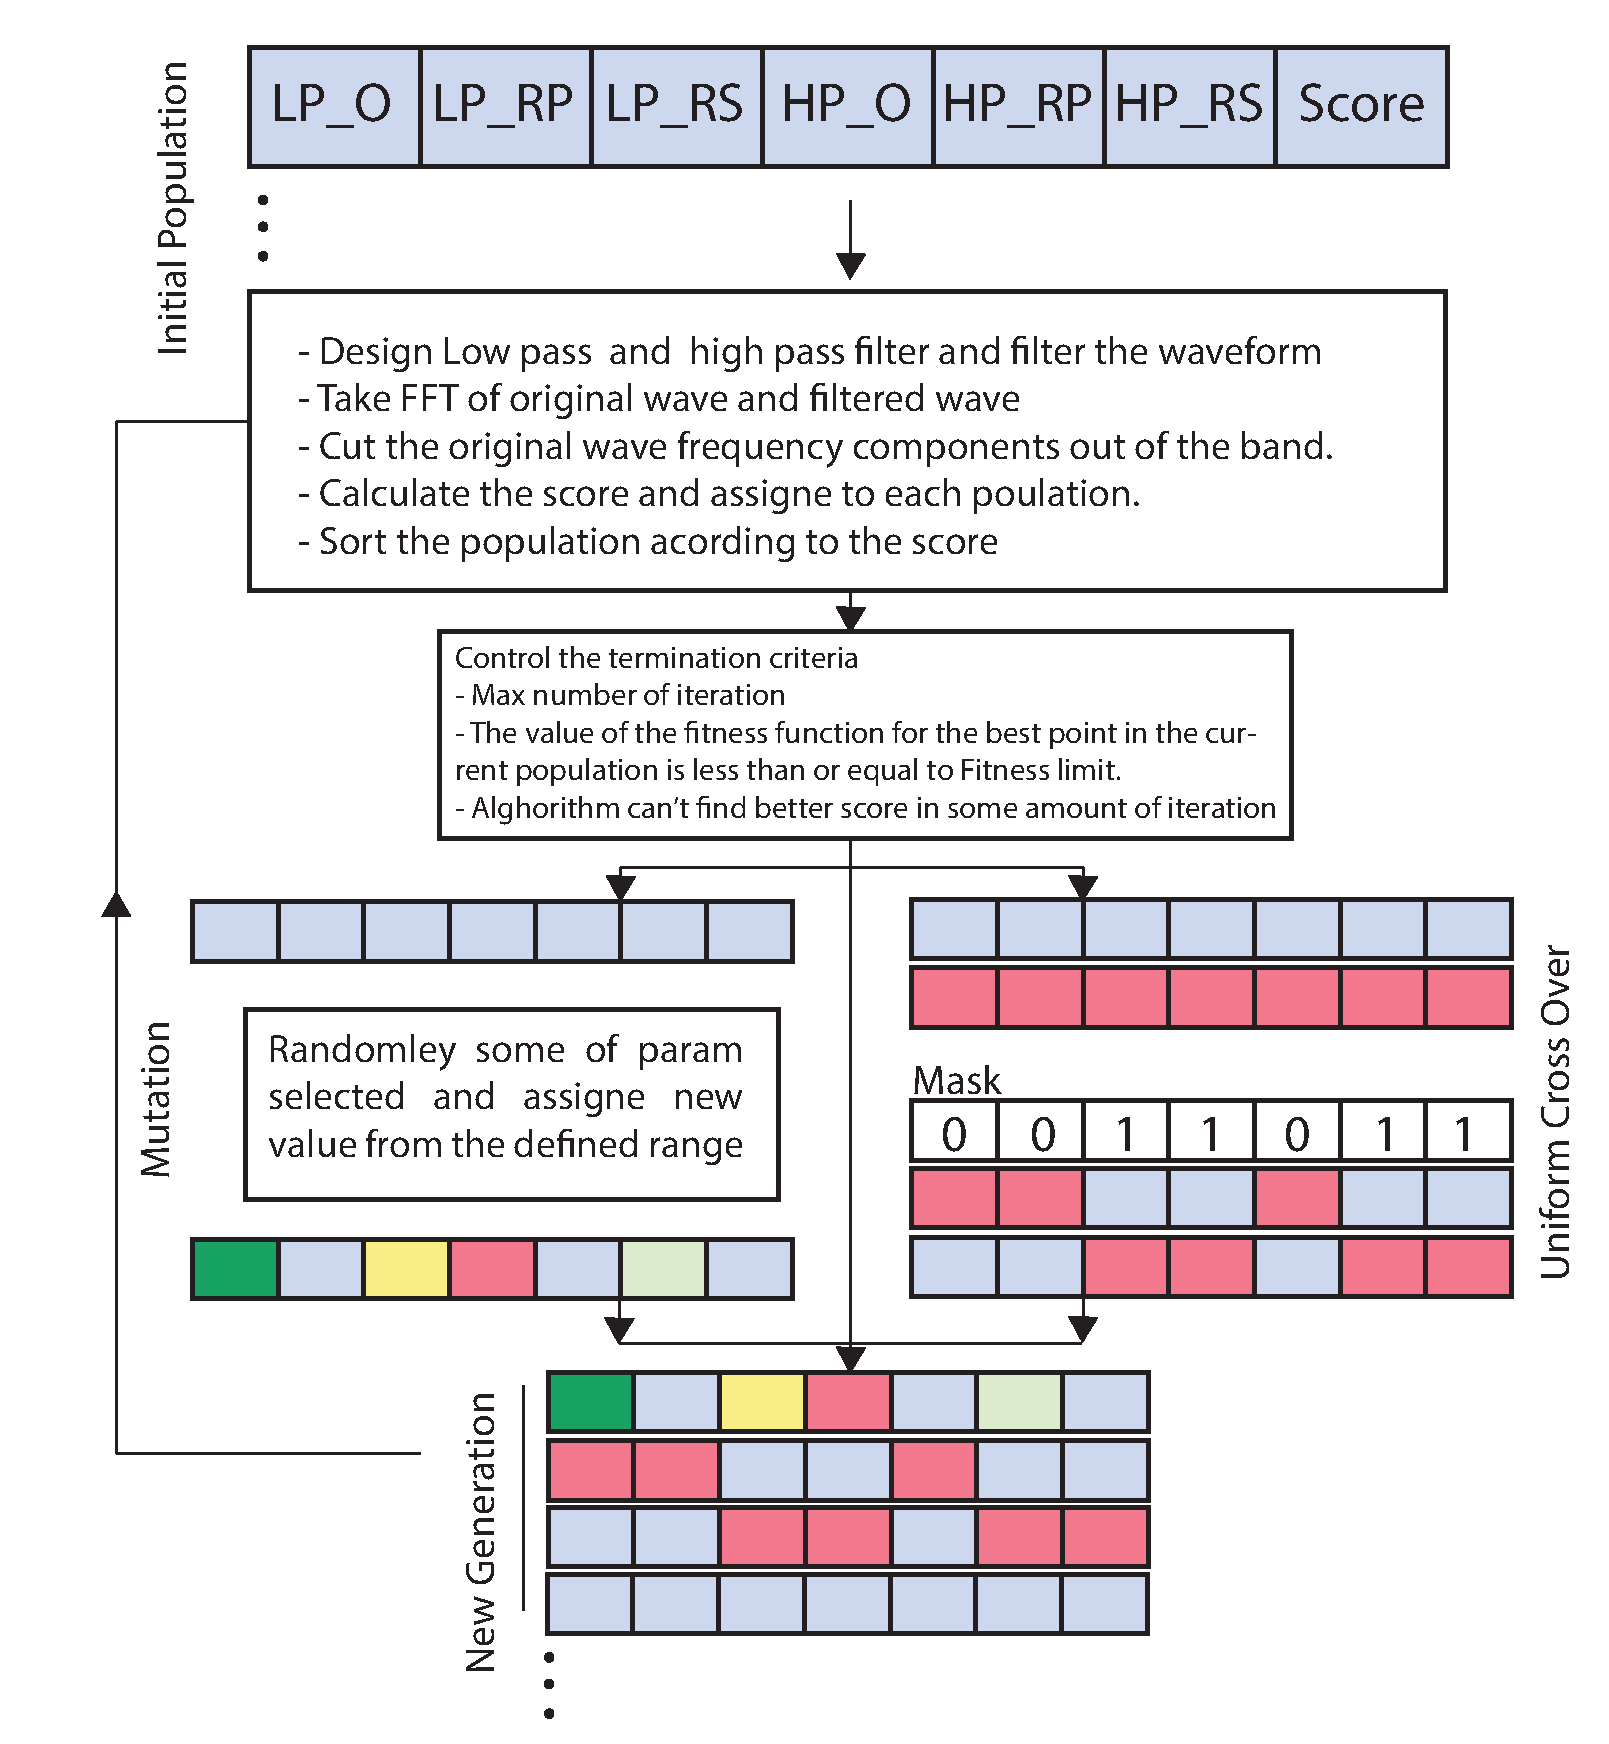
\includegraphics
    	[width=\textwidth]
    	{figures/pdf/figure7.pdf} 
    \caption{GA optimization process}
\end{figure*}

\subsection{White noise definition}

We started to optimize the parameters based on tests on white noises. All numerical signal processing procedures make assumptions about the time series outside of the recorded segments. Time-domain filtering programs assume that the time series is zero on either side of the segment of data being filtered, and frequency-domain filtering using a discrete Fourier transform, as in the FFT, assumes that the time series is periodic, with period equal to the length of the data segments extended with zeros or truncated to a number of points equal to a power of two. 

\citet{Converse-1992} suggest the below equation to zeropad the initial and end of the waveform. 

\begin{equation}
	T{_z{_p{_a{_d}}}} = \frac{1.5n}{f_c}
\end{equation}

Where $T(sec)$ is the total length of zeros to be added to the record, $n$ (an integer) is the order of the Butterworth filter, and $f_c$ is the corner frequency. In this study we deal with different kind of filter and different filtering order, nevertheless the effect of abrupt cut of data is not negligible. \citet{Boore_2005} showed that zero padding assuming the Butterwoth filter order is 4, gives trustable wave form in the sense of numerical problem. Practically it is not possible to filter the waveform with corner frequency of 0 Hz. After \citet{Trifunac_1971}  many networks in order to do baseline correction, high pass filter the waveform  with 0.05 Hz corner frequency ( e.g. cosmos-format). Even though for numerical models, theoretically achieving very close numbers to zero is possible, we wanted to make all analysis consistent for data and synthetic. We choose $f_c= 0.05$ Hz as a smallest highpass corner frequency. So the added time will be 120 s. We add 60 sec of zero pads before and after the data. We defined the 60 white noises with maximum 50 Hz frequency. The total time of data is 100s, which with zero pad part totally will be 220s. We also used Gaussian window ($\alpha$=4) according to equation (7) to taper the data. 

\begin{equation}
\omega{_({_n{_)}}} = e ^ {\frac{-1}{2}(\alpha \frac{n}{\frac{N}{2}})^2}
\end{equation}

Figure 8 shows one the waveforms.

\begin{figure}
    \centering
    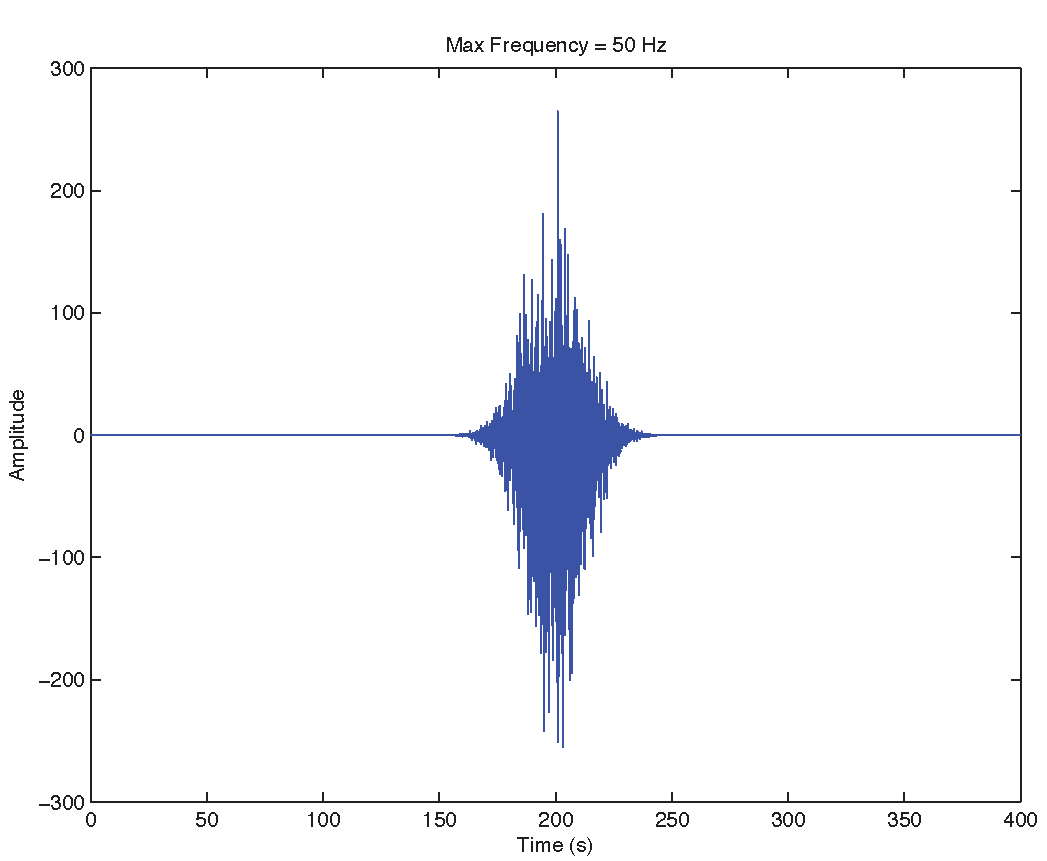
\includegraphics
        [width=\mycolumnwidth]
    	{figures/pdf/figure8.pdf} 
    \caption{Test white noise (\textcolor{red}{time is not correct)}}
\end{figure}


